% !TEX program = xelatex
\documentclass[a4paper]{exam}
\usepackage{amsmath}
\usepackage{stmaryrd}
\usepackage{amsthm}
\usepackage[left=1.8cm,right=1.8cm,top=2.2cm,bottom=2.0cm]{geometry}
\usepackage[UTF8]{ctex}
\usepackage{enumerate}
\usepackage{fancyhdr}
\usepackage{xpatch}
\usepackage{graphicx} 
\usepackage{float} 
\usepackage{subfigure} 
\usepackage{amsfonts}
\usepackage{mathtools}
\usepackage{framed}
\usepackage{multicol}
\usepackage{minted}
\usepackage{fontspec}
\usepackage{float}
\usepackage{tikz}
\usepackage{alltt}
\usepackage{multicol,comment}
\usepackage{biblatex}
\usepackage{amssymb}
\addbibresource{04-discussion.bib}
\usetikzlibrary{automata,positioning}
\usepackage[section]{placeins}
\makeatletter

\printanswers


\AtBeginDocument{\xpatchcmd{\@thm}{\thm@headpunct{.}}{\thm@headpunct{}}{}{}}
\makeatother

\pagestyle{fancy}
\renewcommand{\baselinestretch}{1.15}
\newcommand{\code}[1]{\texttt{#1}}
\usepackage{paralist}
\let\itemize\compactitem
\let\enditemize\endcompactitem
\let\enumerate\compactenum
\let\endenumerate\endcompactenum
\let\description\compactdesc
\let\enddescription\endcompactdesc

% shorten footnote rule
\xpatchcmd\footnoterule
  {.4\columnwidth}
  {1in}
  {}{\fail}
\title{CS 131 Compilers: Discussion 4: More on Syntax-Directed Translation \& Semantic Analysis}
\author{\textbf{杨易为}~~\textbf{吴凌云}~~\textbf{樊雨鑫} \\ \texttt{ \{yangyw,wuly2,fanyx\}@shanghaitech.edu.cn}}

\begin{document}
\maketitle
\section{Syntax-Directed Translation}
In Syntax-Directed (语法制导) Definitions, a Production Rule $A \rightarrow \alpha_{1} \alpha_{2}$ is related to a set of Semantic Rules, which give relations of Attributes of nodes on that Production Rule.

A. syn $=f\left(\alpha_{1} . x, \alpha_{2} . x\right) ; \alpha_{1} . i n=g(A . x)$

The evaluation of the Dependency graph requires a topology sort to assure that for Semantic Rule $b=f\left(c_{1}, c_{2}, \ldots, c_{n}\right)$, it must be evaluated after Rules for $c_{1}, c_{2}, \ldots, c_{n}$

$\begin{array}{ll}\text { Production } & \underline{\text { Semantic Rules }} \\ {D} \rightarrow T L & \text { L.in = T.type } \\ T \rightarrow \text { int } & \text { T.type = integer } \\ T \rightarrow \text { real } & \text { T.type = real } \\L \rightarrow L_{1}, \text { id } & L_{1}. \text {in }=\text { L.in, addtype(id.entry,L.in) } \\ L \rightarrow \text { id } & \text { addtype(id.entry,L.in) }\end{array}$

\begin{figure}[htbp]
  \centering
  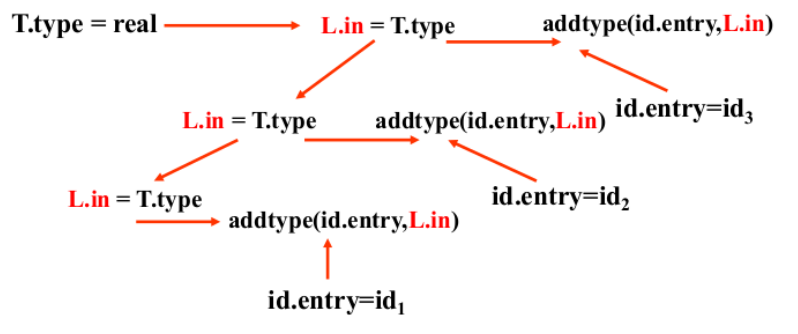
\includegraphics[width=0.4\columnwidth]{./img/CSc.png}
\end{figure}
\begin{enumerate}
  \item \textbf{S-Attributed Definitions} only use Synthesized Attributes. Semantic Action is to put the action in at the end.
  \item \textbf{L-Attributed Definitions} require that in each Production Rule $A \rightarrow \alpha_{1} \alpha_{2} \ldots$ with Semantic Rule $b \rightarrow f\left(c_{1}, c_{2}, \ldots, c_{n}\right):$
        \begin{enumerate}
          \item $b$ is a Synthesized Attribute of $A, \mathrm{OR}$
          \item $b$ is an Inherited Attribute of $\alpha_{j}$, which depends no more than Attributes of $A, \alpha_{1}, \ldots, \alpha_{j-1}$
        \end{enumerate}
        For an Inherited Attribute of $\alpha_{j}$, put the action just before $\alpha_{j}$
\end{enumerate}

\subsection{Left Recursion Elimination}
When there are Left Recursions in the decorated Production Rules, and we want to conduct Top-Down Parsing, we will need to correctly eliminate them by:
$$A \rightarrow A_{1} Y\{\mathrm{~A} . \mathrm{a}=\mathrm{g}(\mathrm{A} 1 . \mathrm{a}, \mathrm{Y} . \mathrm{y})\}$$
$$A \rightarrow X\{\mathrm{~A} . \mathrm{a}=\mathrm{f}(\mathrm{X} . \mathrm{x})\}$$
$$\Downarrow$$

$$A \rightarrow X\left\{\mathrm{~A}^{\prime} .\right. \text{in }\left.=\mathrm{f}(\mathrm{X} . \mathrm{x})\right\} A^{\prime}\left\{\mathrm{A} . \mathrm{a}=\mathrm{A}^{\prime} .\right.\text{syn }\}$$

$$A^{\prime} \rightarrow Y\left\{\mathrm{~A} 1^{\prime} .\right.\text{in }=\mathrm{g}\left(\mathrm{A}^{\prime} .\right.\text{in, }\left.\left.\mathrm{Y} . \mathrm{y}\right)\right\} A_{1}^{\prime}\left\{\mathrm{A}^{\prime} .\right.\text{syn }=\mathrm{A}^{\prime} .\text{syn }\}$$

$$A^{\prime} \rightarrow \varepsilon\left\{\mathrm{A}^{\prime} .\right.\text{syn }=\mathrm{A}^{\prime} .\text{in }\}$$

\subsection{TopLevelDeclList implementation in ChocoPy}
\begin{minted}[mathescape, linenos]{c++}
top_level_decl : top_level_decl var_def {
                  $$ = combine($1, $2);
               }
               | top_level_decl func_def {
                  $$ = combine($1, $2);
               }
               | top_level_decl class_def {
                  $$ = combine($1, $2);
               }
               | top_level_decl assign_stmt {
                  $$ = combine($1, $2);
               }
\end{minted}

\section{Scope}
From today on, we step into a new topic: semantics. In ChocoPy project II, we have to implement the semantic checker and type checker. We will briefly introduce the type system and introduce the type system in ChocoPy. We cast analysis on the grammar from CFG and do as many checks as possible, during which we mark something like type, scope, and runtime garbage collector so that they can do better in runtime.
\subsection{Dynamic Scoping}
A global identifier refers to the identifier associated with the most recent environment and is uncommon in modern languages. In technical terms, this means that each identifier has a global stack of bindings and the occurrence of an identifier is searched in the most recent binding.

\begin{minted}[mathescape, linenos]{c}
/* Since dynamic scoping is very uncommon in the familiar languages, we consider the 
 * following pseudo code as our example. It prints 20 in a language that uses dynamic
 * scoping. */ 
int x = 10;
// Called by g()
int f() {
   return x;
} 
// g() has its own variable named as x and calls f()
int g() {
   int x = 20;
   return f();
}
main() {
  printf(g());
}
\end{minted}
\subsection{Lexical Scoping}

\textbf{Scoping} refers to the issue of matching identifier declarations \cite{identifier} with its Uses. The \textbf{Scope} of an identifier is the portion of a program where it is accessible.
\begin{enumerate}
  \item Same identifier may refer to different things in different portions.
  \item Different scopes for same identifier \textbf{Do Not} overlap.
  \item Usually, search for \textbf{local} definition first, and if not found, goto its parent Scope.
\end{enumerate}

\subsubsection{Python Scoping}

In python, we have 4 kinds of scopes and their life cycle, which is called \textbf{LEBG}. Notice that every scope maintains its namespace, which is literally a bunch of map of identifiers.

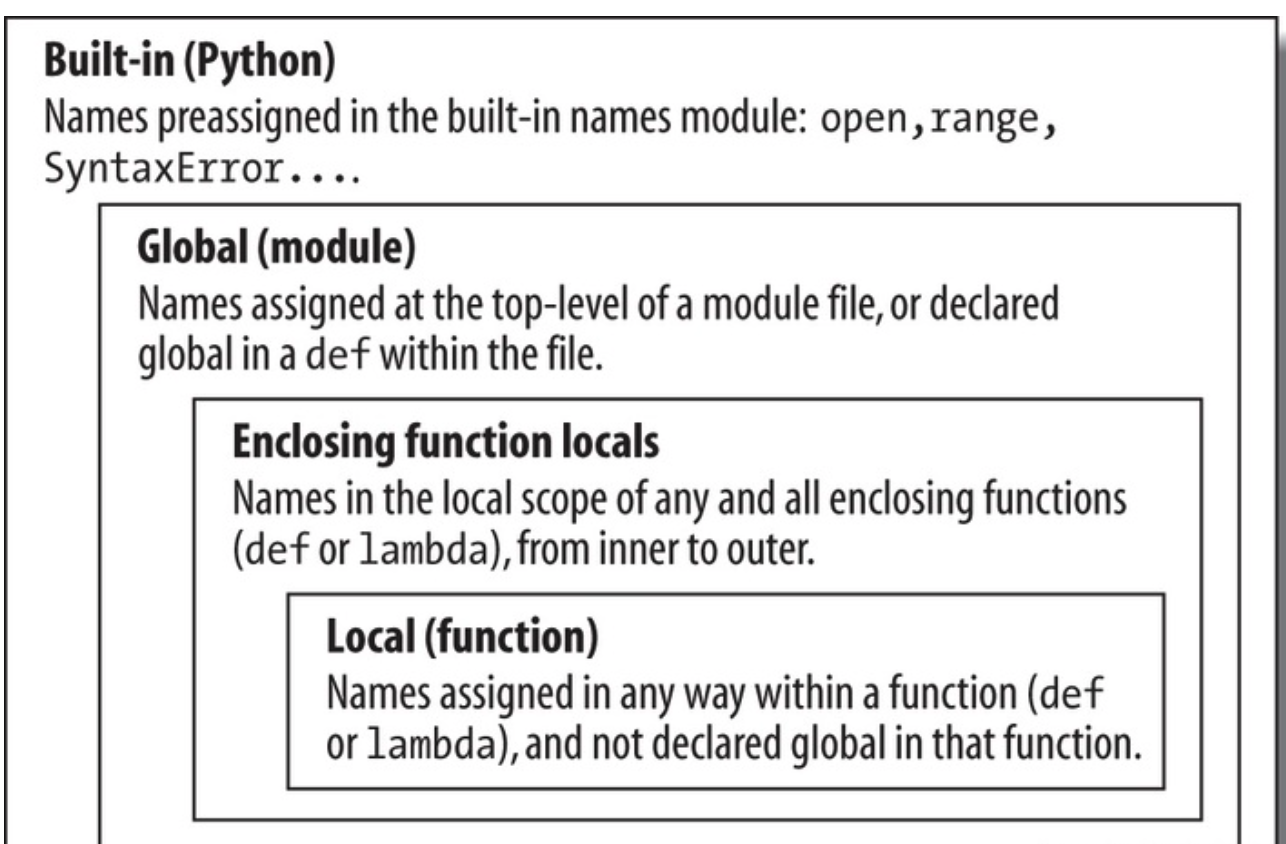
\includegraphics[width=10cm]{img/python_scope.png}
\begin{enumerate}
  \item \textbf{L}ocal scope,  that is, the temporary variables defined in the function, when the function ends, the life cycle of the variable ends.

  \item \textbf{E}nclosed (closure, the local scope of the nested parent function), that is, the local variables of the outer function of the closure, the end of the outer function, the end of the life cycle of the variable.
  \item \textbf{G}lobal (global variables), that is, variables defined at the module level, the module is destroyed, the life cycle of the variable will end.
  \item \textbf{B}ulit-in (built-in function) is the python interpreter, the virtual machine built-in variables.
\end{enumerate}

Here we put a benign testcases and adversarial testcases
\begin{enumerate}
  \item  The benign one
        \begin{minted}[mathescape, linenos]{bash}
      +--------------------------+
      |        +---------------+ |
      | def foo|():            | |
      |   +----+               | |
      |   | x = 1              | |
      |   |          +-------+ | |
      |   | def inner|():    | | |
      |   |   +------+       | | |
      |   |   | return x + 1 | | |
      |   |   +--------------+ | |
      |   | x = 3              | |
      |   | print inner()      | |
      |   +--------------------+ |
      +--------------------------+
\end{minted}

        This inner is a closure(lambda function). The way closures are implemented in Python is to hold a pointer to an external namespace (which can be interpreted as a dictionary).
        \\
         What's the result of the following output?
        \begin{minted}[mathescape, linenos]{python}
def make_averager():
    count = 0
    total = 0
    def averager(new_value):
        nonlocal count, total
        count += 1
        total += new_value
        return total / count
    return averager

averager = make_averager()
print(averager(10))
print(averager(11))
\end{minted}
        \begin{solution}
10.0\\
10.5
        \end{solution}
  \item The malicious one
        \begin{minted}[mathescape, linenos]{python}
def f0(): // NameError: name 'a' has'nt been defined
  a = 123
  def g():
      exec("print(a)")
  g()

def f1(): // print("123\n123")
  a = 123
  def g():
      exec("print(a)")
      print(a)
  g()

def f2(): // NameError: name 'a' has'nt been defined
  a = 123
  def g():
      print(eval("a"))
  g()

def f3(): // print("123\n123")
  a=123
  def g():
      print(eval("a"))
      print(a)
  g()
\end{minted}
        The \textbf{eval} is another story. The built-in \textbf{eval} function, which evaluates a string as a Python expression(运行字符串中存储的指令). The grammar is listed below.
        \begin{minted}[mathescape, linenos]{python}
  eval(source[, globals[, locals]]) -> value
\end{minted}
        Where \textbf{source} is a Python expression or code object return by a function \textbf{compile()}, global is dictionary and locals is any mapped object.

\end{enumerate}
\subsubsection{Doc is not enough, show me your code}

The code is from CPython\cite{CPython}, a interpreter in C to speed up python.
\begin{minted}[mathescape, linenos]{c}
static PyObject *
builtin_eval(PyObject *module, PyObject *const *args, Py_ssize_t nargs)
{
    PyObject *source;
    PyObject *globals = Py_None;
    PyObject *locals = Py_None;

    source = args[0];
    globals = args[1];
    locals = args[2];
/* ... Checks */
int r = _PyDict_ContainsId(globals, &PyId___builtins__);
if (r == 0) {
    r = _PyDict_SetItemId(globals, &PyId___builtins__,
                          PyEval_GetBuiltins());
}
if (r < 0) {
    return NULL;
}

if (PyCode_Check(source)) {
    if (PySys_Audit("exec", "O", source) < 0) {
        return NULL;
    }

    if (PyCode_GetNumFree((PyCodeObject *)source) > 0) {
        PyErr_SetString(PyExc_TypeError,
            "code object passed to eval() may not contain free variables");
        return NULL;
    }
    return PyEval_EvalCode(source, globals, locals);
}

PyCompilerFlags cf = _PyCompilerFlags_INIT;
cf.cf_flags = PyCF_SOURCE_IS_UTF8;
str = _Py_SourceAsString(source, "eval", "string, bytes or code", &cf, &source_copy);
if (str == NULL)
    return NULL;

while (*str == ' ' || *str == '\t')
    str++;

(void)PyEval_MergeCompilerFlags(&cf);
result = PyRun_StringFlags(str, Py_eval_input, globals, locals, &cf);
Py_XDECREF(source_copy);
return result;
}
\end{minted}

What is the above code impls of scoping, evaluation at which time and how \textbf{eval()} interact with input strings?

\begin{solution}
The eval will be evaluate after the scope analyzer. If \texttt{print(a)} exists, it will add \texttt{a} to the \texttt{locals}. The \texttt{Globals} and \texttt{locals} are passed into the scope.
\end{solution}
\subsubsection{The Scope of Decorator}
When we analyze the calling process of a unknown procedure. The decorator in Python is to make the grammar nice and neat. If you work for Python Open Source community, you must have heard of PEP8 \cite{pep8}. Utilizing Decorator and other grammar sweet is a good way, and also may give you a insight to understand others' reason of writing so. For a general view, a language is all about its grammar sweet.

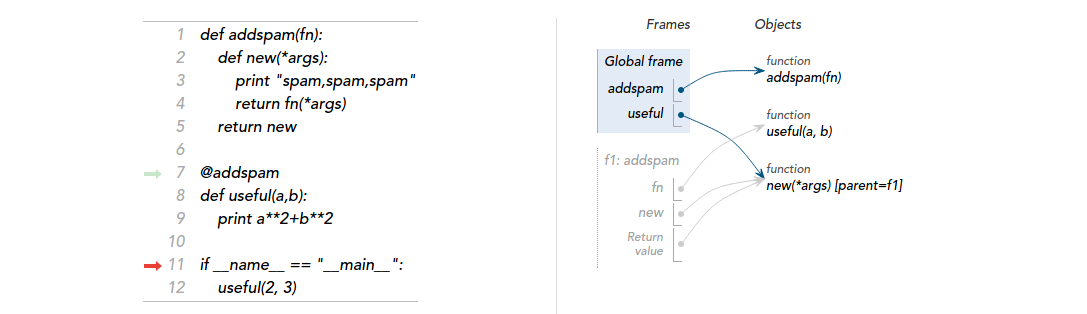
\includegraphics[width=15cm]{./img/decorator.png}



\subsubsection{Make good use of Python Scoping}
\begin{minted}[mathescape, linenos]{python}
class IntermediateNumber(ABC):
  # class internal namespace, can be shared through the lifetime of the class
  numbers: ClassVar[List[int]]
  digits: int
  def __init__(self, number: Union[List[int], int], digits: int, from_natural: bool):
      self.digits = digits
      if from_natural:
          self.numbers = self.from_natural(number)
      else:
          # builtin function
          if isinstance(number, int): # convert int to List[int]
              numbers = [int(c) for c in str(number)]
          else:
              numbers = number
          # class function
          if not self.check(numbers):
              raise ValueError(f'number not valid: {numbers}')
          self.numbers = numbers
      if digits - 1 > len(self.numbers):
          self.numbers = [0] * (digits - 1 - len(self.numbers)) + self.numbers
  # internal function for stringify
  def __str__(self):
      return f'{self.__class__.__name__[:3]}({"".join(map(str, self.numbers))}){self.custom_str()}'
  # type checking, rhs is callable.
  def check(self, number: List[int]) -> bool:
      return True
  def __add__(self, rhs: IntermediateNumber):
      assert isinstance(self, rhs.__class__)
      return self.add(rhs)
  def __sub__(self, rhs: IntermediateNumber):
      assert isinstance(self, rhs.__class__)
      assert self.to_natural() >= rhs.to_natural()
      return self.sub(rhs)
  # rhs is callable.
  # generate from natural number
  @abstractmethod
  def from_natural(self, natural: int) -> List[int]:
      pass
  # convert back to natural number
  @abstractmethod
  def to_natural(self) -> int:
      pass
  @abstractmethod
  def add(self, rhs: IntermediateNumber):
      pass
  @abstractmethod
  def sub(self, rhs: IntermediateNumber):
      pass
\end{minted}

Better for libraries' unit tests and fuzzing tests.

\subsubsection{Python interpretor is not as strong as you think}
Not every is picklable, a serialization technique when packing tedious python object. We need it because when we need to have multiprocessing or networking stuffs while because of GIL, python is too too too slow. What is not picklable?
The lambda functions along with functions and classes defined in the \texttt{\_\_main\_\_} module, which is the function in the global scope or in a class function.

How to solve it?

Cloud-pickle.
\begin{minted}[mathescape, linenos]{python}
from .cloudpickle import (
    _extract_code_globals, _BUILTIN_TYPE_NAMES, DEFAULT_PROTOCOL,
    _find_imported_submodules, _get_cell_contents, _is_importable,
    _builtin_type, _get_or_create_tracker_id,  _make_skeleton_class,
    _make_skeleton_enum, _extract_class_dict, dynamic_subimport, subimport,
    _typevar_reduce, _get_bases, _make_cell, _make_empty_cell, CellType,
    _is_parametrized_type_hint, PYPY, cell_set,
    parametrized_type_hint_getinitargs, _create_parametrized_type_hint,
    builtin_code_type,
    _make_dict_keys, _make_dict_values, _make_dict_items,
)
\end{minted}
\section{Type System}
A type is a set of values together with a set of operations on those values. A language's type system specifies which operations are valid for which types. Jane street has a debate of dynamical type and static type. \cite{janestreetcode}


The notion of "correctness" often depends on what the programmer has in mind, rather than what the representation would allow.

Most operations are legal only for values of some types
\begin{enumerate}
  \item Doesn't make sense to add a function pointer and an integer in C
  \item It does make sense to add two integers
  \item But both have the same assembly language implementation: \texttt{movl y, \%eax;  addl x, \%eax}
\end{enumerate}

\subsection{Type System for a Toy Language}
Define \cite{cs164lec12} a really easy typeof to connect with operational semantic for cool. we only will consider the following subset grammars.
\begin{verbatim}
  defn(I,T,[def(I,T)| _])
  defn(I, T, [def(I1,) | R]) :- dif(I, I1), defn(I, T, R).
  typeof(X, T, Env) :- defn(X, T, Env).
  \end{verbatim}
\texttt{\_} means "don't care" or "wildcard", \texttt{I} is defined to have type \texttt{T} if the environment list starts with such a definition, or if \texttt{I} isn't the same as the identifier in the first def but matches the next suitable definition further down the list.
\begin{alltt}
  e : ID | int
  | [ ((e ,)* e)?  ] /* list */
  | \(\lambda\) ( ID , e )
  | e '+' e
  | e '<<' e
  | e '//' e
  | cast(e,e)
\end{alltt}

Begin with two typing rules.
\begin{verbatim}
  typeof(X, int,_) :- integer(X).
  typeof(X, T, Env) :- defn(X, T, Env).
\end{verbatim}

\begin{enumerate}
  \item Write a typing rule such that the type of an empty list is unbounded (e.g \texttt{[\_]}).

        \begin{solution}
\begin{verbatim}   
typeof ([],[_], _)
\end{verbatim}
        \end{solution}

  \item  Write a typing rule such that the type of a list is [T], where all list elements are of type T.

        \begin{solution}
\begin{verbatim}
typeof ([E|R], [T], Env) :- typeof (E, T, Env), typeof (R,[T], Env)
\end{verbatim}
        \end{solution}

  \item Write a typing rule such that the type of a lambda is $T1->T2$, where $T2$ is the return type and $T1$ is the type X is bound to within the body of the lambda.

        \begin{solution}
\begin{verbatim}
typeof(lambda(X, E), T1->T2, Env) :- typeof(E, T2, [def(X, T1)| Env])
\end{verbatim}
        \end{solution}

  \item Write a typing rule such that the type of $L + R$ is int when L and R are both of type int.

        \begin{solution}
\begin{verbatim}
typeof(L + R, int, Env) :- typeof(L, int, Env), typeof(R, int, Env)
\end{verbatim}
        \end{solution}

  \item Write a typing rule such that the type of $L // R$ is \texttt{[T]} when L and R are both of type \texttt{[T]}.

        \begin{solution}
\begin{verbatim}
typeof(L // R, [T], Env) :- typeof(L, [T], Env), typeof(R, [T], Env)
\end{verbatim}
        \end{solution}
        
  \item Write a typing rule such that the type of $L << R$ is T2 when L is of type T1 -> T2 and R is of type T1.
  \begin{solution}
  \begin{verbatim}
typeof(L << R, T2, Env) :- typeof(R, T1, Env), typeof(L, T1->T2,Env)
\end{verbatim}
  \end{solution}
  \item Write a typing rule such that the type of $cast(L,R)$ is $T1 -> T2$ when L is of type $T1$ and R is of type $T2$.

        \begin{solution}
\begin{verbatim}
typeof(cast(L, R), T1 -> T2, Env) :- typeof(L, T1, Env), typeof(R, T2, Env)
\end{verbatim}
        \end{solution}

\end{enumerate}

Then we can get the reverse operation to infer type using \texttt{typeof}:
\begin{enumerate}
  \item \begin{verbatim}
typeof(f << g, T, [def(f, int->[int]), def(g, int)]).
  \end{verbatim}

        \begin{solution}
\begin{verbatim}
T = [int]
\end{verbatim}
        \end{solution}
  \item \begin{alltt}
typeof(\(\lambda\)(x, x // x) << [1], T, []).
  \end{alltt}

        \begin{solution}
\begin{verbatim}
T = [int]
\end{verbatim}
        \end{solution}
  \item \begin{alltt}
typeof(\(\lambda\)(x, x + x) << [1], T, []).
  \end{alltt}

        \begin{solution}
false
        \end{solution}
  \item \begin{alltt}
typeof(\(\lambda\)(x, x + x) << 1, T, []).
  \end{alltt}

        \begin{solution}
int
        \end{solution}
  \item \begin{alltt}
typeof(\(\lambda\)(x, x + x) + 1, T, []).
  \end{alltt}
        \begin{solution}
false
        \end{solution}
  \item \begin{alltt}
typeof(\(\lambda\)(x, x // x) << [\(\lambda\)(x, x // x)], T, []).
  \end{alltt}

        \begin{solution}
\begin{verbatim}
[[T1]->[T1]]
\end{verbatim}
        \end{solution}
  \item \begin{alltt}
typeof(\(\lambda\)(x,\(\lambda\)(y, cast(x,y))) << [\(\lambda\)(x,\(\lambda\)(y, cast(x,y)))],T, []).
  \end{alltt}

        \begin{solution}
\begin{verbatim}
(T3->[(T1->(T2->(T1->T2)))]->T3)
\end{verbatim}
        \end{solution}

\end{enumerate}

\subsection{Type Checking Rules}
The goal of type checking is to ensure that operations are used with the correct types, enforcing the intended interpretation of values.

\subsubsection{Another toy type checking system in lambda calculus}

This language has only two types, ${\bf Bool}$ and ${\bf Int}$, and terms can be represented by numbers, ${\rm True}$, ${\rm False}$, ${\rm if}\ b\ {\rm then}\ u \ {\rm else}\ v$, and addition and subtraction (of course, multiplication and division can be added, but for convenience we will only use (plus or minus).

We have some derivation rules.

\begin{enumerate}
  \item any integer of type ${\bf Int}$.
  \item ${\rm True}$ and ${\rm False}$ are of type ${\bf Bool}$.
  \item if $a$, $b$ are of type ${\bf Int}$, then $a+b$ is of type ${\bf Int}$ and $a-b$ is of type ${\bf Int}$.
  \item If $b$ is of type ${\bf Bool}$ and $u,v$ are of type $T$ (note that $T$ is not fixed), then ${\rm if}\ b\ {\rm then}\\ u {\rm else}\ v$ is of type $T$.
\end{enumerate}

For example, $14$ belongs to ${ Int}$ and $9$ belongs to ${ Int}$, so $14+9$ belongs to ${Int}$, which is deduced from rule 3.

Notice that there are "illegal" terms in this language, such as ${ if}\ 13\ { then}\ 5\ { else}\ 4$, which are obviously of incorrect type. We call all items with a certain type well-typed

This language is not very useful, but it allows us to recognize some notation in type theory.

Narrating rules in words can easily go wrong when the system is more complex, so it is necessary to narrate them in a formal language.

Use $a:T$ to indicate that the item $a$ belongs to type $T$, and $\vdash a:T$ to indicate the fact that "we can infer that $a:T$". $\vdash$ is called a turnstile (a direct translation), and later we will add "context" to its left side, but now it is always empty.

We can write the derivation rule in the following form.
$$
  \cfrac{v{\rm\ is\ a\ number}}{\vdash v:{\bf Int}}{\rm\tiny(NUM)}
  \qquad\cfrac{}{\vdash {\rm True}:{\bf Bool}}{\rm\tiny(TRUE)}
  \qquad\cfrac{}{\vdash {\rm False}:{\bf Bool}}{\rm\tiny(FALSE)}
$$
$$
  \cfrac{\vdash a:{\bf Int}\quad\vdash b:{\bf Int}}{\vdash a+b:{\bf Int}}{\rm\tiny(PLUS)}
  \qquad\cfrac{\vdash a:{\bf Int}\quad\vdash b:{\bf Int}}{\vdash a-b:{\bf Int}}{\rm\tiny(MINUS)}
  \quad\cfrac{\vdash b:{\bf Bool}\quad\vdash u:T\quad\vdash v:T}{\vdash ({\rm if}\ b\ {\rm then}\ u\ {\rm else}\ v):T}{\rm\tiny(IF)}
$$

Here we have a horizontal line indicating the derivation from top to bottom, with several preconditions above the line (or maybe none, like the (TRUE) rule here), and a conclusion below the line. The marker to the right of the horizontal line indicates the name of the rule. This represents an \textbf{inference rule}.

The advantage of this is that we can prove a conclusion by overlaying one horizontal line after another. For example, if we want to prove that $({\rm if\ True\\ then}\ (14+5)\ {\rm else}\ 3):{\bf Int}$, we can write it like this.
$$
  \cfrac{
  \cfrac{}{\vdash {\rm True}:{\bf Bool}}{\rm\tiny(TRUE)}
  \quad\cfrac{
  \cfrac{14{\rm\ is\ a\ number}}{\vdash 14:{\bf Int}}{\rm\tiny(NUM)}
  \quad\cfrac{5{\rm\ is\ a\ number}}{\vdash 5:{\bf Int}}{\rm\tiny(NUM)}
  }{\vdash (14+5):{\bf Int}}{\rm\tiny(PLUS)}
  \quad\cfrac{3{\rm\ is\ a\ number}}{\vdash 3:{\bf Int}}{\rm\tiny(NUM)}
  }{\vdash ({\rm if\ True\ then}\ (14+5)\ {\rm else}\ 3):{\bf Int}}{\rm\tiny(IF)}
$$

Before we introduce the imputation rules, let's look at the concepts of free variable and bound variable.
A variable $x$ in a term is said to be free if and only if it does not match some abstraction. For example, $y(\lambda x . x)$ is a term in which $y$ is free and $x$ is bounded. Variables with the same name can also be both free and bounded, for example $\textcolor{red}{x}(\lambda x . \textcolor{green}{x})$ where the red $x$ is free and the green $x$ is bounded. Note that the position after $\lambda$ does not count as $x$, it is just a notation here.
Specifically, a single item of $x$ where $x$ is free; $t_{1} t_{2}$ does not change whether each variable is free or not; $\lambda x . t$ binds all $x$ in $t$, without affecting other variables.
By analogy, a free variable is a global variable and a bound variable is a local variable.

\begin{enumerate}
  \item $\alpha$-conversion
        As mentioned above, we can change the name of a local variable, for example, $\lambda x . x y$ to $\lambda a . a y$, or $\lambda x . (\lambda x . x)$ becomes $\lambda y . (\lambda x . x)$ (because the $x$ in it is not free, so it doesn't need to be changed). But it's not free, for example, we can't change $\lambda x . x y$ to $\lambda y . y y$.
        So our requirement is roughly: in $\lambda x . M$, if all $y$ in $M$ are bounded (or don't appear at all), then we can turn it into $\lambda y . (M[x:=y])$. Such a transformation is called $\alpha$-conversion, and we generally consider the terms that can be transformed into each other by $\alpha$-conversion to be the same (syntactically equivalent, i.e., three, rather than equivalent in the sense of being reducible to the same term).
        The necessity of $\alpha$-conversion is that we sometimes need to rename other variables in $M$ when computing $M[x:=N]$, for example, $(\lambda y \cdot x y)[x:=(y z)]$ should become $(\lambda a \cdot(y z) a)$ instead of $(\lambda y \cdot(y z) a). \lambda y \cdot(y z) y)$. The latter would cause $y$ to be bound incorrectly when it should be free.
        There is also something called $\eta$-conversion, which presumably means that when $x$ does not appear free in $M$, $\lambda x . M x \equiv M$. This is generally unnecessary, but it's not usually a problem to add.
  \item $\beta$-reduction
        The reduction rule is called $\beta$-reduction, and it is also simple: $(\lambda x . M) N \twoheadrightarrow M[x:=N]$. Sometimes it is also written as $\twoheadrightarrow{ } _ {\beta}$.

        Two terms $M, N$ are said to be equal if they are reducible to the exact same term, denoted as $M=N$ or $M={ } _ {\beta} N$
\end{enumerate}

\subsubsection{$\lambda_\to$ system \cite{barendregt1992lambda}}

\begin{enumerate}
\item Definition

This is a very simple but not so simple type system, unlike the previous toy language which can only be used as an example, where the properties are almost immediately obvious and the proofs are trivial.

Types are also simple: a type is defined as $T::=A\mid T_1\to T_2$, which means that a type is either a primal name or of the form $T_1\to T_2$.

The type $A\to B$ is called \textbf{arrow type}, which intuitively represents the function from $A$ to $B$. This is right-bound, that is, $A\to B\to C$ means $A\to(B\to C)$.

\item Derivation rules

The derivation rule is actually quite simple: the type of the individual variables is required to be chinned; if $M:A\to B,N:A$ then $(MN):B$ (i.e., the function is applied). The derivation of $\lambda x.M$ then looks like this: if we additionally charm $x:A$ when $M:B$, then we get $(\lambda x. M):(A\to B)$.
$$
  \cfrac{(x:A)\in\Gamma}{\Gamma\vdash x:A}{\rm\tiny(VAR)}
  \qquad\cfrac{\Gamma\vdash M:(A\to B)\quad\Gamma\vdash N:A}{\Gamma\vdash (MN):B}{\rm\tiny(APP)}
  \qquad\cfrac{\Gamma,x:A\vdash M:B}{\Gamma\vdash (\lambda x.M):(A\to B)}{\rm\tiny(ABS)}
$$
The $\Gamma, x:A$ in the (ABS) rule refers to expanding the context, complementing $x:A$, and if there was already $x:C$ in $\Gamma$ then remove that (meaning, the local variables inside shield the local variables outside).

Three Inference Rules are all it takes to get a useful type system that is still beautiful. For example, we can derive it like this.
$$
  \cfrac{\cfrac{x:A,y:B\vdash x:A}{x:A\vdash(\lambda y.x):(B\to A)}}{\vdash (\lambda x.\lambda y.x):(A\to B\to A)}
$$
Both of these steps use the (ABS) rule. An easy way to write them is to leave out the Context and $\vdash$ symbols and cross them out when abstracting over a variable. For example
$$
  \cfrac{\cfrac{\cfrac{\{x:A\}^2\quad\{y:B\}^1}{x:A}}{(\lambda y.x):(B\to A)}\small1}{(\lambda x.\lambda y.x):(A\to B\to A)}\small2
$$
Since you can't type a strike through, please imagine changing the brackets to a strike through (

That is, cross out $y:B$ at step 1 (because it is out of context after this step) and cross out $x:A$ at step 2 of the derivation.

\item Some properties

There are some properties (theorems) in the $\lambda_\to$ system, such as

\begin{enumerate}
  \item if $\Gamma\vdash M:A$, then all the free variables in $M$ appear in $\Gamma$, in particular, if $\vdash M:A$, then $M$ contains no free variables.
  \item if $\Gamma \vdash M:A, \Gamma\subseteq\Gamma_1$, then $\Gamma_1\vdash M:A$.
  \item if $\Gamma\vdash M:A,M\twoheadrightarrow _ \beta M'$, then $\Gamma\vdash M':A$ (the converse does not hold, e.g. $(\lambda y.\lambda x.x)(yy)$ has no type).
  \item if $\Gamma\vdash M:A,\Gamma\vdash M':A',M={ }_\beta M'$, then $A\equiv A'$.
\end{enumerate}
\end{enumerate}
\subsubsection{Curry-Howard isomorphism \cite{softwarefoundation}}

\textbf{Curry-Howard Isomorphism} establishes a correspondence between type systems and formal logic systems (types are propositions, programs are proofs).

The $\lambda_\to$ type system then corresponds to propositional logic. Consider that each type $A$ corresponds to a proposition (also denoted by $A$) and that the type $A\to B$ corresponds to the proposition "$A$ implies $B$". A term corresponds to a proof of the proposition.

In this case, since $A$ implies $B$ is equivalent to "if you have a proof of $A$, you can construct a proof of $B$", it is equivalent to "given a term of type $A$, apply this function to obtain a term of type $B$ " is equivalent.

As an example, two of the axioms in a system of propositional logic that uses only implication are
$$A\to (B\to A);$$
$$(A\to(B\to C))\to((A\to B)\to(A\to C))$$
Corresponding to the type, this can be given by the following term.
$$
  \lambda x.\lambda y.x$$
$$  \lambda x.\lambda y.\lambda z.xz(yz)
$$
Separation rules
$$
  \cfrac{\vdash A\to B\quad\vdash A}{\vdash B}
$$
is also exactly the application.

Contexts can also correspond: a context $\Gamma$ in the type system corresponds to a logical system that says all types in $\Gamma$ as preconditions. The (ABS) rule also corresponds to the theorem that $A\vdash B$ is then $\vdash A\to B$.

When we later extend the type system, we can use it to correspond to more complex logic systems, such as higher-order propositional logic, predicate logic, etc.

Here is another small question: what should $\lnot A$ correspond to in propositional logic?

In $\lambda_\to$, we can extend the type system by adding the type $\bot$. It means "empty type", i.e. there is no item of this type, which corresponds to a logically permanent false proposition. And we can add a rule: $\cfrac{\Gamma\vdash x:\bot}{\Gamma\vdash x:A}$. Simply put, if we get a value of the empty type, we can get a value of any type. The logical equivalent is to say that if we get a contradiction then we can derive any conclusion.

Then we can define $\lnot A=A\to\bot$.

Then a new problem arises: we cannot get such a term: $\lnot(\lnot A)\to A$. Without such a term, the converse is not possible (the essence of the converse method is to prove that the negation of the original proposition is false, thus proving that the original proposition is true). So after adding $\bot$ $\lambda_\to$ in fact corresponds to \textbf{intuitionist logic}, or what is called \textbf{constructionist logic}, because we can essentially only construct a proof, and cannot do so by the law of the row ($A\lor\lnot A$), the law of the quadratic reciprocal inverse ($\lnot(\lnot A)\to A$), unless We keep such type of terms in Context (i.e., set as axioms).

\subsubsection{Type Checking in ChoocoPy \cite{cs164chocopy}}
ChocoPy start with the following environment:

$$O( len )=\{ object \rightarrow int ; arg \}$$
$$O( print )=\{ object \rightarrow< None >; arg \}$$
$$O( input )=\{\rightarrow str \}$$
$$M( object,\_\_init\_\_ )=\{ object \rightarrow< None >; self \}$$
$$M( str,\_\_init\_\_ )=\{ object \rightarrow< None >; self \}$$
$$M( int,\_\_init\_\_ )=\{ object \rightarrow< None >; self \}$$
$$M( bool,\_\_init\_\_ )=\{ object \rightarrow< None >; self \}$$

It will iterate to check all the not checked variable.

$$O, M, \perp, \perp\quad \vdash \text { program }$$
\hline $$  \vdash \text { program }$$


For function def, the easier with the function def. First check the return type if it's defined. Then check the arguments and the body whether return type is right. 
$$
  \begin{tabular}{l}
    $T=\left\{\begin{array}{l}T_{0}, \quad \text { if -> is present, } \\ \text { <None>, otherwise. }\end{array}\right.$                                   \\
    $O(f)=\left\{T_{1} \times \ldots \times T_{n} \rightarrow T_{0} ; x_{1}, x_{2}, \ldots, x_{n} ; v_{1}: T_{1}^{\prime}, \ldots, v_{m}: T_{m}^{\prime}\right\}$   \\
    $n \geq 0 \quad m \geq 0$                                                                                                                                       \\
    $ O\left[T_{1} / x_{1}\right] \ldots\left[T_{n} / x_{n}\right]\left[T_{1}^{\prime} / v_{1}\right] \ldots\left[T_{m}^{\prime} / v_{m}\right], M, C, T \vdash b $ \\
    \hline$$ O, M, C, R \vdash \operatorname{def} f\left(x_{1}: T_{1}, \ldots, x_{n}: T_{n}\right) \llbracket \rightarrow T_{0} \rrbracket^{?}: b$$
  \end{tabular}
$$
\subsection{Type Inference}

Types of expressions and parameters need not be explicit to have static typing. With the right rules, might infer their types.

The appropriate formalism for type checking is logical rules of inference having the form. cool is a statically typed

\begin{minted}[mathescape, linenos]{scala}
  doh() : Int { (let i : Int <- h in { h <- h + 2; i; } ) };
\end{minted}
Here the \texttt{doh} can be inferred as the type should be int even \texttt{doh()} does not have a type hint.
\subsubsection{Type Inference in ChoocoPy}
The type of list created by a non-empty display is the least upper bound (denoted $\sqcup$ ) of the types of its elements, where the relevant type relation is $\leq_{a}$, rather than pure subtype.
$$
  \begin{tabular}{l}
    $n \geq 1$                                        \\
    $O, M, C, R \vdash e_{1}: T_{1}$                  \\
    $O, M, C, R \vdash e_{2}: T_{2}$                  \\
    $\vdots$                                          \\
    $O, M, C, R \vdash e_{n}: T_{n}$                  \\
    $T=T_{1} \sqcup T_{2} \sqcup \ldots \sqcup T_{n}$ \\
    \hline$O, M, C, R \vdash\left[e_{1}, e_{2}, \ldots, e_{n}\right]:[T]$
  \end{tabular}
$$
Here are two groups of examples
\begin{enumerate}
    \item bool+int vs. str+int
$False + 8 \quad \# \textcolor{green}{OK}$\\
$"False" + 8\quad \# \textcolor{red}{ERROR}$\\
 \item The object list can be to infer the type object in the second case. however, int list is not able to make equal to object list.
$\mathrm{x}:[$ object $]=$ None\\
$\mathrm{x}=[3, \mathrm{x}] \quad \# \textcolor{green}{OK}$\\
$x = [3]\quad\quad \# \textcolor{red}{ERROR}$
\item 
\begin{minted}[mathescape]{python}
class A(object):
    a:B=None
    def __init__(self:A,other:B)->object:
        a=other
class B(object):
    pass
class C(B):
    pass
a:A=None
b:A=None
c:B=None
d:C=None
a=A(b)
b=A(c)
a=b
\end{minted}
 Subclass can be used to function arg passing.
\end{enumerate}
\subsection{Type Unification}
To unify two type expressions is to find substitutions for all type variables that make the expressions identical. The algorithm that follows treats type expressions as objects (so two type expressions may have identical content and still be different objects). All type variables with the same name are represented by the same object. It generalizes binding by allowing all type expressions (not just type variables) to be bound to other type expressions.

\begin{figure}[htbp]

  \centering
  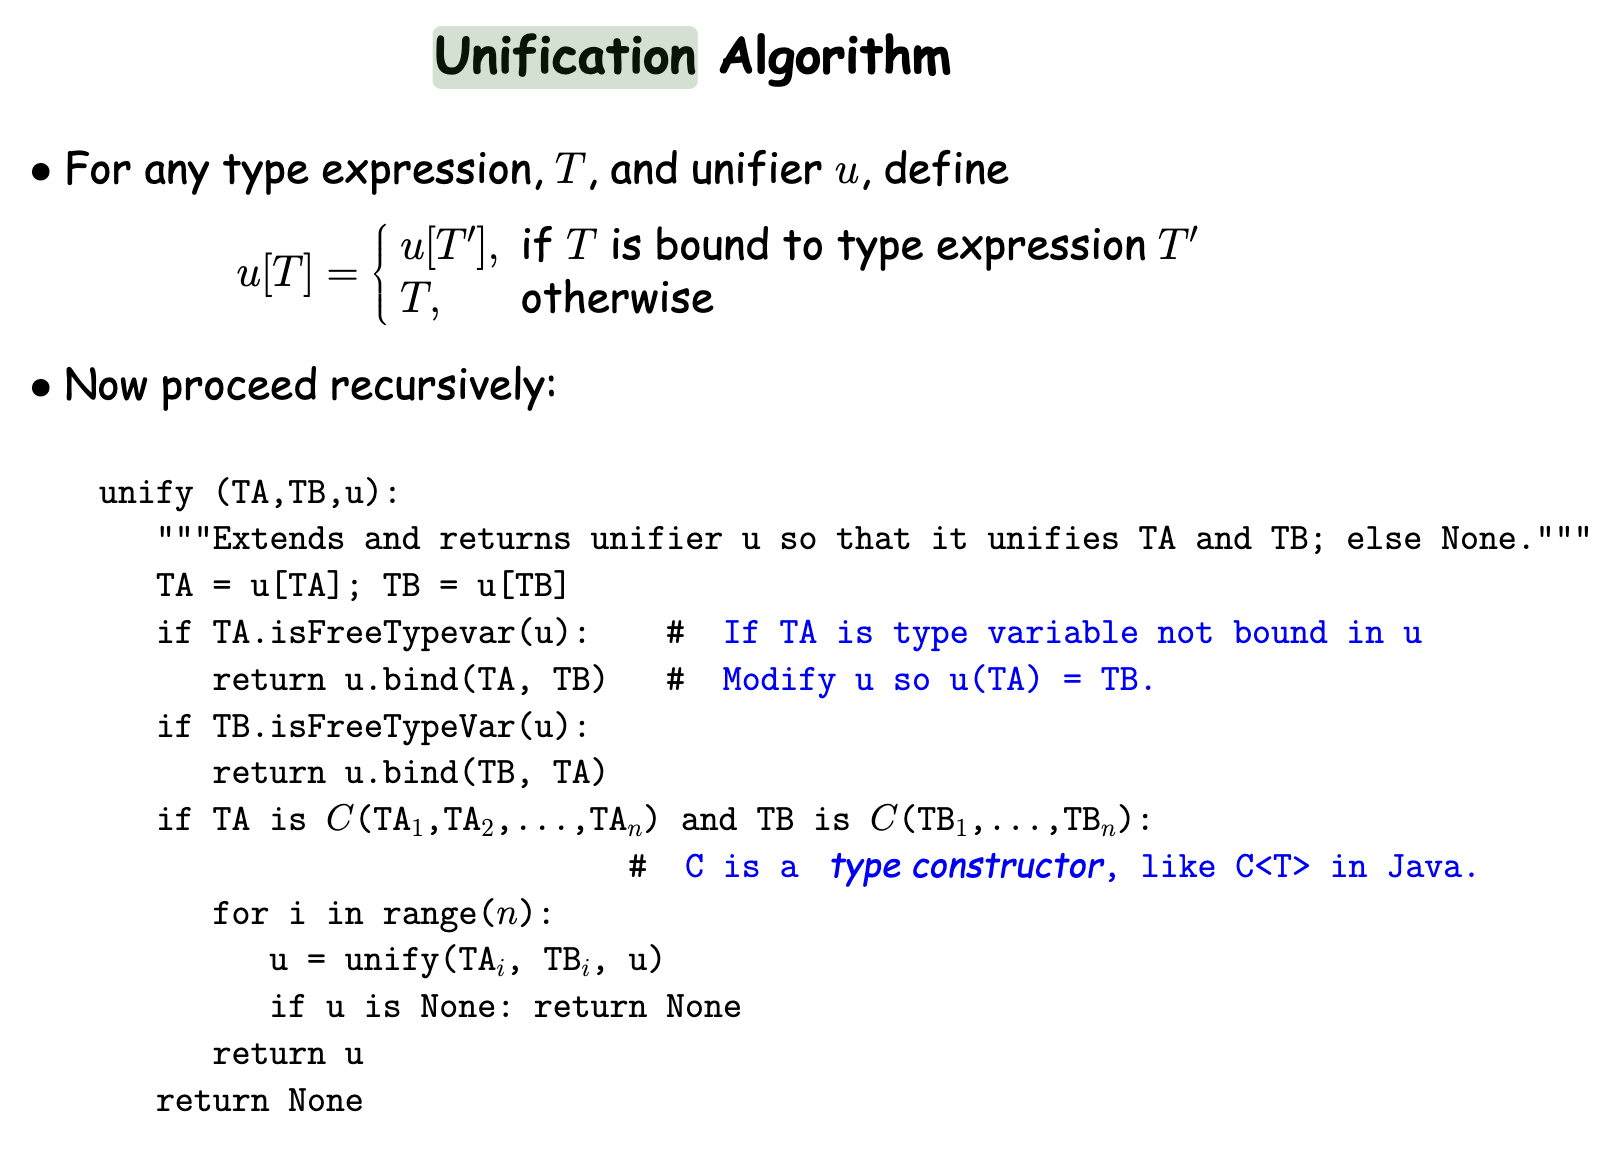
\includegraphics[width=10cm]{img/unification.png}
  \subsubsection{Type Unification in ML}
\end{figure}

\begin{figure}[htbp]
  \centering
  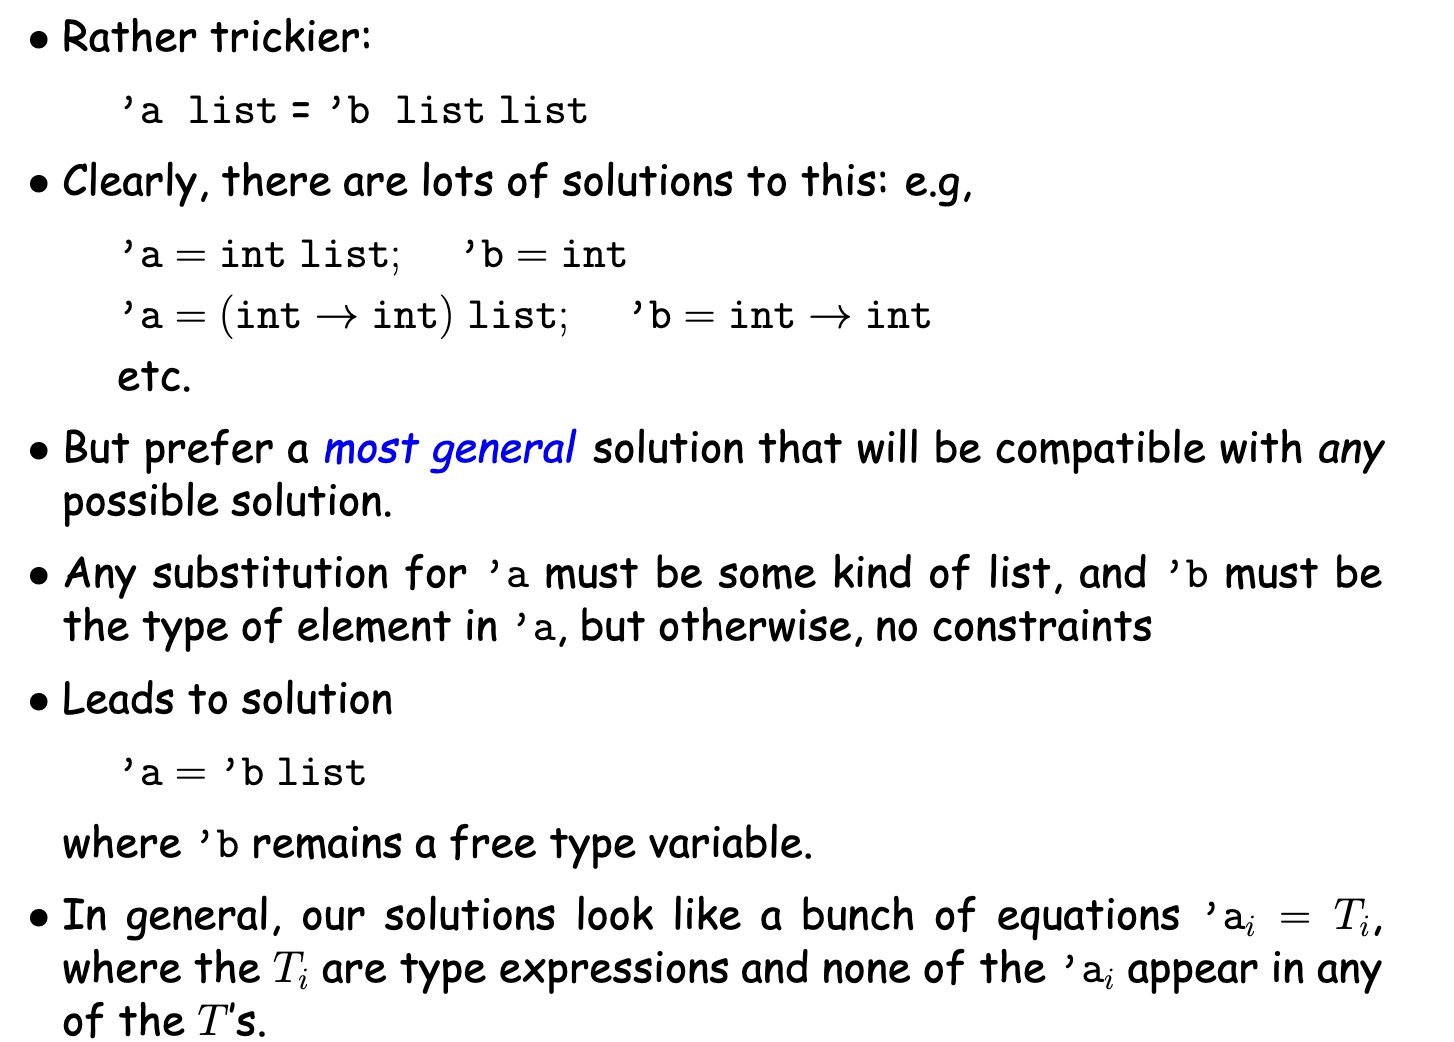
\includegraphics[width=10cm]{./img/type_unification.png}
\end{figure}

\begin{figure}[htbp]
  \centering
  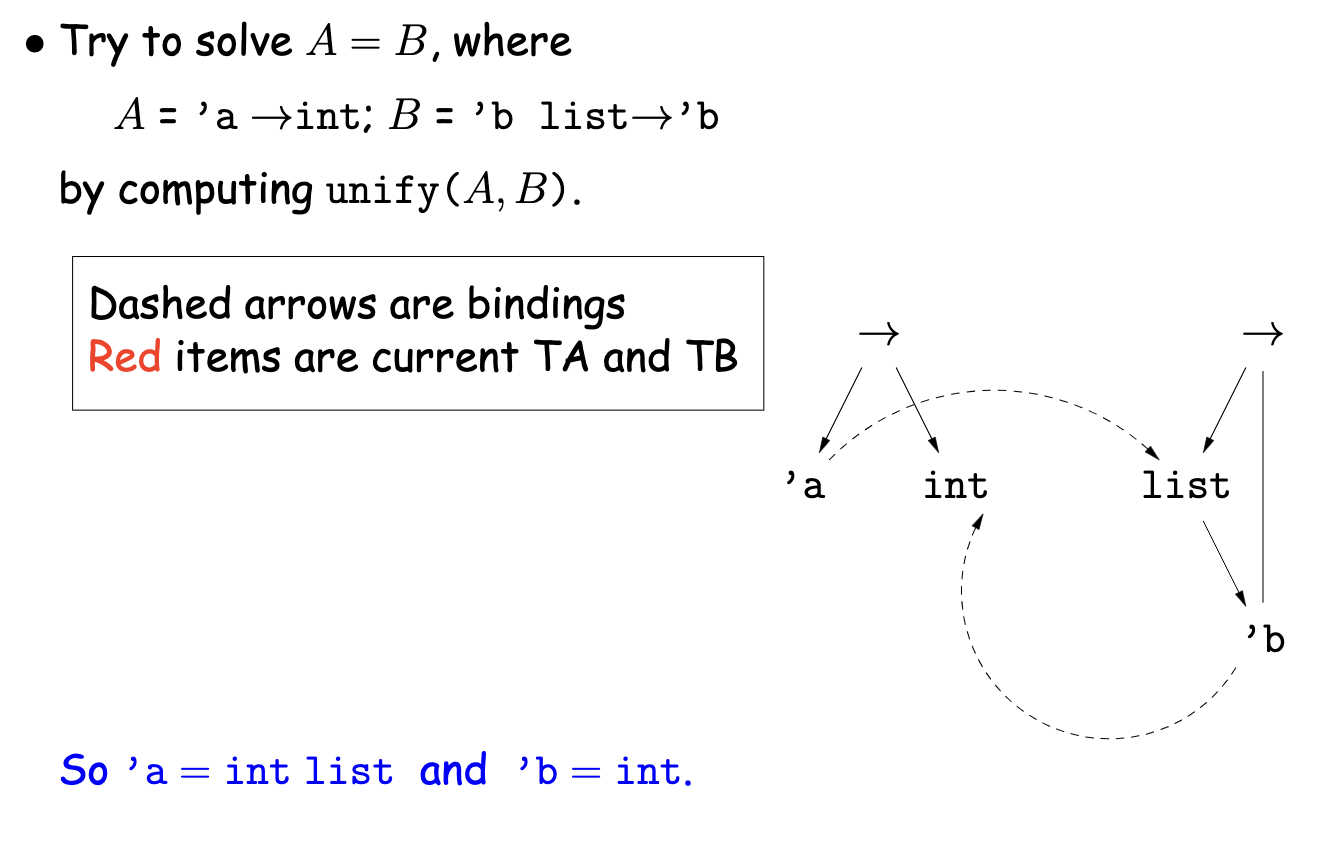
\includegraphics[width=10cm]{./img/type_eg.png}
\end{figure}

\begin{figure}[htbp]
  \centering
  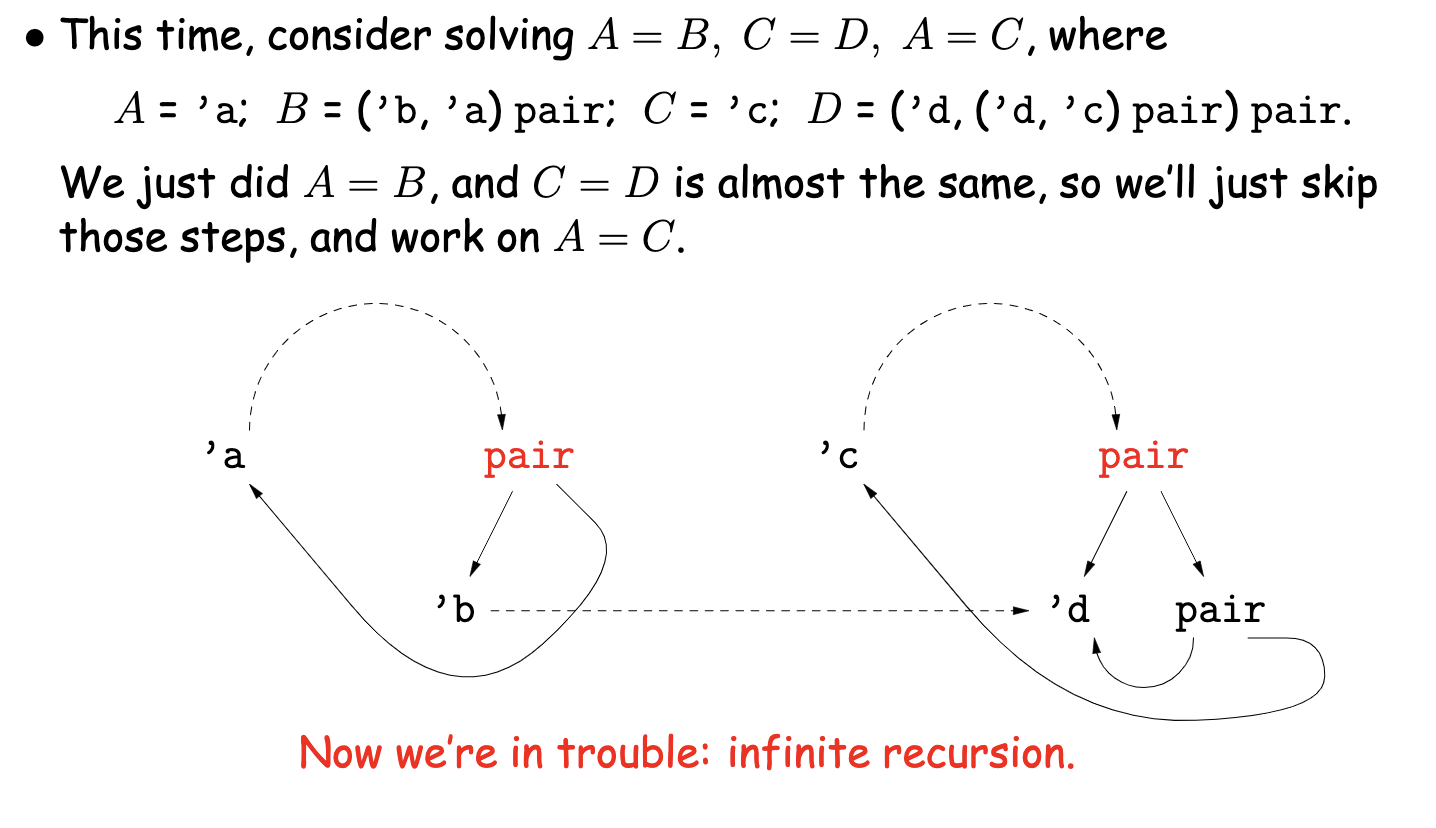
\includegraphics[width=10cm]{./img/recursive_type.png}
\end{figure}
  \subsubsection{Typecases in ChocoPy}
\begin{minted}[mathescape]{python}
class A(object):
    a:int = 42
class B(A):
    b:bool = True
    def __init__(self:"B")->object:
        self.a = 38
class C(B):
    c:bool = True
    def __init__(self:"C")->object:
        self.a = 32
b:A=None
d:str=input()
b=A()
if d=="sb":
    b=C()
else:
    b=B()
print(b.a)
\end{minted}
\printbibliography

\end{document}
